The purpose of this thesis was to consider whether there was evidence for a dynamic yield-precipitation relationship for corn in Ontario and Iowa. Given that the empirical results suggested that this relationship was in fact dynamic, the secondary aim was to analyze how neglecting to consider this dynamic relationship would affect the estimated actuarially fair premium rates. The results showed that failing to account for the dynamic yield-precipitation relationship led to biased premium rate estimates. Finally, the yield model was used to estimate future potential yields under climate change so that the potential climate effects on corn yield could be considered. In both Iowa and Ontario, the results showed that the yield variance is expected to increase given climate change. The mean yield in Ontario is expected to slightly increase given climate change, while a slight decrease is expected in Iowa.

\section{Summary}

To accomplish the purpose and objectives of this research project, the literature on corn yield modelling and weather was reviewed in order to determine the independent variables that were most appropriate for use in the yield model. A list of potential variables to be included in the model was developed. Given the agronomic complications which arise due to growth stages and interdependent weather effects, the exact choice of variables and variable timing was not obvious. A total of 49 different linear models were tested for both Iowa and Ontario, with the precipitation thresholds excluded. The choice of model to use in each location was selected based on the model sum squared error, as well as on the interpretation and significance of the coefficients.

Once the model variables were selected, the analysis focused on the nature of the yield precipitation relationship over time. This relationship was approximated using threshold levels, which is essentially assumes that there exists some `ideal' precipitation range. Both a two threshold and a one threshold model were considered. Each of these models was estimated using two methods, one of which was a simplification of the other and relied on the additional assumption that the degree of spatial correlation in the error term would not be significantly altered by the threshold levels. In addition to looking at Iowa and Ontario as a whole, subsets of the counties in Ontario were considered due to expected heterogeneity between counties.

In order to allow for the dynamic precipitation yield relationship, the threshold levels were time dependent. Each threshold was represented as a linear function of time based on two parameters. This linear function determined the levels of the thresholds for each year included in the data set. The potential threshold values were constrained such that the thresholds were never larger or smaller than the maximum and minimum precipitation realizations included in the data set respectively. The lower threshold was also constrained to be smaller than or equal to the upper threshold throughout the study period. Within these constraints, various threshold parameters were considered. In the two threshold model, this resulted in four parameters which could be modified, while in the one threshold model, two parameters could be modified. The model was estimated given a particular parameter combination (and therefore a particular combination of threshold levels over time), and the model sum squared error was saved in a matrix. The combination of parameters which led to the smallest sum squared error was selected as the optimal threshold parameter solution for the location in question. 

The parameters controlling the direction and magnitude of change in the threshold levels over time were the main results of interest. The two threshold models all showed the lower threshold to be increasing through time in all locations. The upper threshold results were not consistent however, and showed the upper threshold to be increasing or decreasing depending on the location and method of estimation. The results from the one threshold model were very consistent. The single threshold model showed the threshold to be increasing through time in all locations considered, and when estimated by both methods. Due to the consistency of the single threshold model results, the single threshold model was used for the remaining analysis. The single threshold model was estimated both by method 1 and method 2, where method 2 was a simplification of method 1 and was much less computationally demanding. The results from method 2 for the one threshold model were very similar to those obtained through method 1 in all locations considered in terms of the threshold parameters selected, the model parameter values, and the model fit. Since the second method was simpler and led to similar results, this method was used for the remaining analysis.

Given that the results suggested that the demand for precipitation during the silking period was increasing for corn in both Iowa and Ontario, the potential effects of assuming a static relationship between yield and precipitation was considered in terms of its effect on the estimated actuarially fair premium rate. In both Iowa and Ontario, given weather simulated from current climate, the use of the static yield model to generate yields resulted in premium rate estimates which were smaller than that estimated based on the dynamic yield model. These differences were found to be statistically significant, implying that not accounting for the dynamic nature of the yield precipitation relationship could lead to underestimation of risk under current climate conditions. Given future simulated weather, the use of the static model led to an overestimation of risk in Iowa, while the estimates were not statistically different under the static versus the dynamic models in Ontario.

In order to consider how potential climate change could impact yield, expected dynamic model yields were calculated based on both the current and future weather data. These expected yields were calculated assuming current agricultural technology given both current and future climate. This was done given the inability to accurately predict long term trends in technological progress. The yield expectations under future climate were calculated given the future precipitation threshold level while those under current climate were calculated given the current threshold level. In Iowa the mean yields were statistically different under climate change in 68 out of the 99 counties at or above the 90\% confidence level, with the average difference in expected yield under climate changed equal to -1.903. The variance was found to be statistically different in 76 out  of 99 counties at or above the 90\% confidence level, and both the variance and mean were found to be statistically different at this confidence level in 59 counties. The average difference in estimated standard deviation was equal to 1.112.  In Ontario 26 out of the 32 counties had statistically different means at the 90\% confidence level or above, while 21 had statistically different variance, and both the mean and variance of the yields were statistically different in 18 counties. The average difference in expected yield was equal to 4.031, and the average difference in variance was equal to 2.128. Therefore, the results found that the precipitation-yield relationship appears to be dynamic, neglecting to account for this relationship can impact the actuarially fair premium rate estimates, and climate change will likely increase yield variance.

 
\section{Implications of Results}

The results suggest that the demand for precipitation has increased over time. They also show that neglecting to account for the dynamic nature of the yield precipitation relationship leads to biased premium estimates, given that the dynamic model is assumed to be correct. Finally, the results showed that if climate were to change in the manner simulated, yield variance would likely increase both in Iowa and Ontario. The mean yields in Ontario could be expected to increase slightly under climate change, while those in Iowa could be expected to decrease slightly.

The increased demand for precipitation over time implies that precipitation will be a limiting yield factor more often now then it was in the past, suggesting that yields could become more variable under climate change. The results are consistent with producers substituting subsidized crop insurance programs for other income risk mitigating strategies in agreement with \citep{kerRMP2016}. The observed increase in precipitation demand is a product of increasing mean yields, but also leads to an increased likelihood of low yield years. 

In both Ontario and Iowa, the precipitation threshold appeared to be increasing through time. However, the starting point and the rate at which the threshold level changed over time was significantly different in Iowa and Ontario. Figure 7.1 shows the levels of the threshold over time in each location from 1950 to 2090.

\begin{figure}
 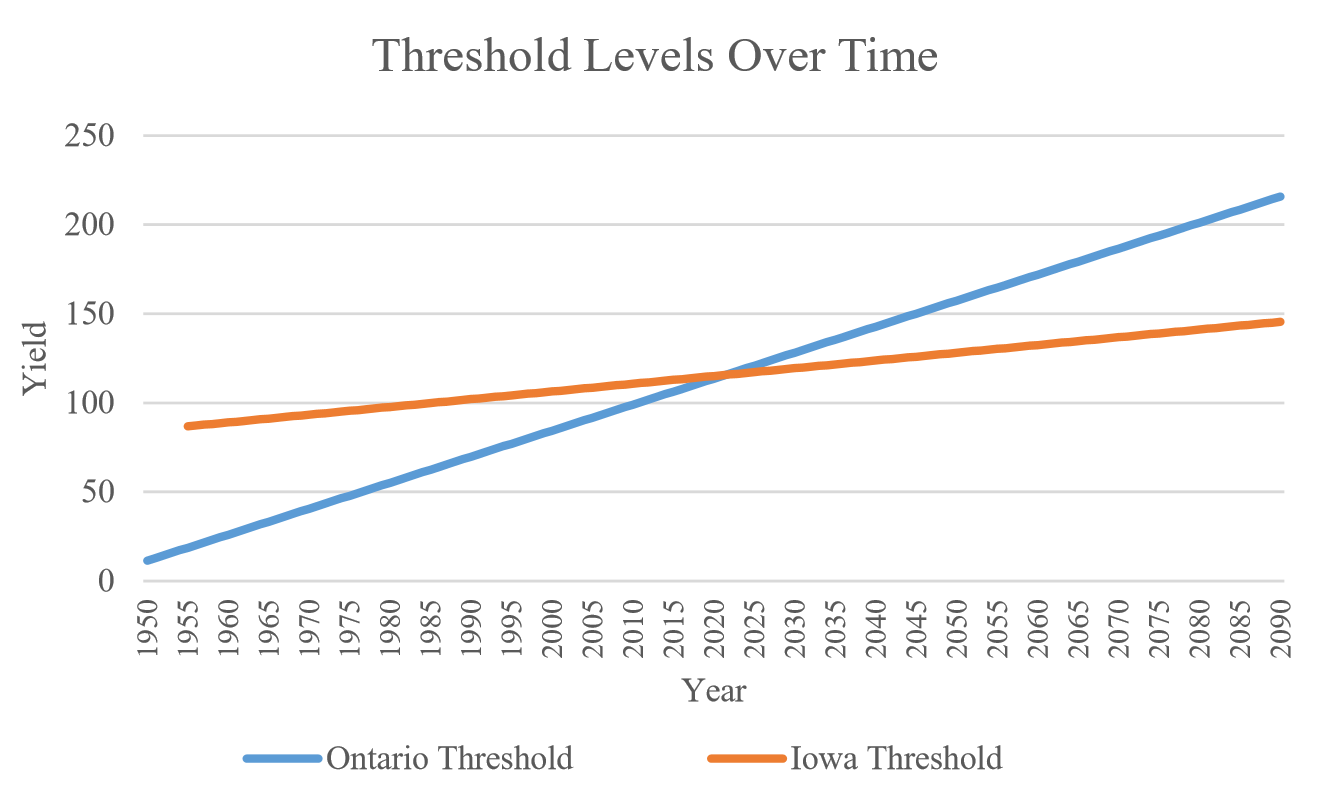
\includegraphics[width=\textwidth]{thresholdlevelstime.png}
    \caption{Threshold Levels Over Time}
 \end{figure}

The results suggest that given the more quickly increasing precipitation threshold, Ontario will be more sensitive to management practices which increase the soil water holding capacity, such as soil rotations, and practices which increase the level of soil organic matter \citep{williams2016soil}. If the increase in demand continues in the future, these sensitivities could become increasingly apparent.

The expected yields under climate change behaved differently in Iowa and Ontario. In both locations, climate change appeared to lead to increased yield variability due to weather. However, in Ontario the mean expected yields increased under climate change while they slightly decreased in Iowa. This is likely attributable to the relative current temperatures in these locations. Iowa is relatively warm in comparison to Ontario. Currently, Iowa tends to receive high $GDD$ accumulation levels over the corn growing season, and is subject to a more significant extreme heat effect. Under climate change, both $HDD$ and $GDD$ increase. Since $HDD$ is already relatively high under current climate the $HDD$ in Iowa increases more than in Ontario and the relative negative temperature effect is greater. Additionally, since $GDD$ does not increase when temperatures are above 29 degrees Celsius, which occurs more commonly in Iowa, the increased temperature under climate change increases the $GDD$ measure more in Ontario than in Iowa. Therefore, the positive heat effect is more substantial in Ontario. This explains why the effect of climate change may be different in the two study locations. The observation of this effect suggests that Ontario, and other relatively northern areas of agricultural production, could be relatively more competitive under climate change.

\section{Further Research}

Consideration of a wider variety of potential climate change scenarios given the dynamic precipitation yield model should be considered. The effect of climate change was considered in only one potential case. Generating yields given a wider variety of scenarios could give a better idea of the potential range of climate change effects on corn yields. Considering how premium rates could develop under these various scenarios would also be of interest.

The large increase in yield per acre over the study period is not unique to corn. Additionally, corn is not the only crop which is primarily rain fed. This problem could therefore apply to other crops in other locations. Additionally, the precipitation effect during the pollination and silking growth stage was the focus of this paper. It is possible that changes in the precipitation effect during other growth stages could also empirically be demonstrated over time. 

Given that the results show that the precipitation demand is increasing over time, the economic viability of irrigation systems could also be changing. Further research could attempt to estimate the profitability of irrigation systems given different climate scenarios. In this way, an estimate of when and where irrigation could become a profitable production choice could be estimated. Additionally, the value of farm management practices which can increase the soil water holding capacity could be considered.

Another point of interest is how specific corn varieties differ in terms of their responses to these types of constraints. Further research could consider what types of corn varieties are the least sensitive to drought conditions as well as to extreme heat. Estimates of the relative cost to the public of insuring these different varieties under various climate scenarios could be computed. 

\section{Policy Recommendations}


The results suggest that precipitation induced yield variability will likely increase, given that precipitation demand appears to be increasing over time, and given that precipitation could become more variable under climate change. If yields become more variable, crop insurance payouts will become more common. This implies that premium rates will likely need to increase in the future. Since the cost is shared with the public, this means that the cost of crop insurance programs may increase. Crop insurance in generally subsidized in order to attempt to increase program participation. However, it has been suggested that due to the lower share of risk held by the producer, subsidized crop insurance could increase the likelihood that the producer will make risky production decisions \citep{kerRMP2016}. Estimating the correlation between subsidy levels and overall yield variability over time could quantify this. Given that climate change may increase yield variability, other methods which can counteract this affect may become important. The potential for the lowering of yield variance over time through decreasing subsidy levels should be considered. 


The results of this thesis show that excessive heat and low precipitation decreases mean yields and increases yield variability, in agreement with \cite{williams2016soil} . 	\cite{lee2015topsoil} found that when precipitation was high, stability was increased in that the yields were not as sensitive to shallow top soil. This suggests that measures to increase soil moisture, such as irrigation, would more likely be beneficial in areas with thinner top soil depths. Conservation practices can decrease the sensitivity of crops to water by increasing the amount of water that can be held in the soil and therefore making it less likely that water will limit yield potentials \citep{IowaSWCS}. Tillage increases the evaporation rate of water from soil and may therefore be detrimental to yields, especially if precipitation becomes more variable or in areas where soils do not retain water well \citep{IowaSWCS}. Deeper soil allows the corn plant to root more deeply, and can decrease it's sensitivity to rain patterns \citep{Guilpart}. Top soil erosion negatively impacts corn yield through the inability to absorb rainfall quickly. This can lead to a higher rate of run off and therefore a decrease in the total amount of water available to the plant \citep{Guilpart}. This suggests policy decisions which encourage producers to maintain soil quality and to increase the level of soil organic carbon content so that they can hold a larger capacity of water and thereby decrease the lilkelihood that precipitation levels will limit yield.  Management practices which support this outcome include no till or reduced till farming, and using compost or cover crops to increase the organic material however the soil type in the region limits the effectiveness of these practices \citep{williams2016soil}.

\section{Main Results and Research Contributions}

The first question to be answered in this thesis was whether the relationship between corn yield and precipitation has changed over time. The results suggest that the level of precipitation required to attain high yields has increased over time in both Iowa and Ontario as expected. Under current climate, the estimated actuarially fair premium rates estimated using the static model were biased down, under the assumption that the dynamic model is correct. Given the future simulated climate, the estimated actuarially fair rates in Iowa were higher when the static model was assumed while in Ontario the resulting premium rates were not significantly different. Finally, based on model averages assuming the A1B climate scenario of the IPCC, the effect of potential climate change on yield relative to current climate and technology levels was considered. In Iowa the yield realizations were slightly higher on average and had slightly lower variance on in the current climate assumption. In Ontario however the average yield appeared to increase under climate change as did the variance. These differences in results are likely due to the difference in current climate between Iowa and Ontario. Based on this research, it appears that an awareness of the changing yield precipitation relationship can have implications for predicting losses for a crop insurer. The demand for precipitation appears to be increasing through time as stated above. If this trend were to continue it could result in an increase in the probability that precipitation will be a limiting factor for yields. This possibility could alter the profitability of irrigation systems and other agricultural technologies, such as drought resistant corn plants. 

This thesis contributes to the literature on corn yield modelling and crop insurance through the consideration of a dynamic relationship between weather variables and corn yield. The use of threshold levels to allow a non linear precipitation-yield effect was not encountered in the literature. Furthermore, the use threshold levels to empirically test whether the yield-precipitation relationship was changing through time was novel. These modifications to the commonly used linear model increase flexibility and suggest the existence of trends which were not previously considered empirically. The differences in the resultant premium estimates when assuming a static versus a dynamic yield precipitation relationship demonstrate the potential practical ramifications of the main result. Finally, the consideration of potential climate effects on expected yields suggested that the effect of climate change on agriculture will likely depend on the underlying distribution of key weather variables under current climate. It appears that climate change will likely increase yield variability in the locations studied. However, mean yields could be expected to increase in the relatively cold Ontario region, while they may decrease in Iowa. This suggests that climate change will likely alter the locations which have comparative agricultural advantage. When temperatures increase, new regions which were previously too cold to be fit for agriculture may become available for use in agricultural production. Therefore, climate change could lead to differences in where agricultural commodities are produced. This thesis empirically tested whether the precipitation-yield relationship had changed through time and concluded that it had. This changing relationship was found to have significant effects on the estimation of the actuarially fair level of crop insurance premium rates. Finally, the climate change scenario simulated suggested that yield variability would increase in both Ontario and Iowa under climate change.


















